\documentclass[a4paper,12pt]{article}

% ==============================
%            ПАКЕТЫ
% ==============================
\usepackage{cmap}
\usepackage[T2A]{fontenc}
\usepackage[utf8]{inputenc}
\usepackage[english,russian]{babel}
\usepackage{hyperref}
\usepackage{multicol}
\usepackage{mathtools}
\usepackage{amssymb}
\usepackage{enumitem}
\usepackage{tikz}
\usepackage{cancel}
\usetikzlibrary{automata, positioning, arrows.meta}
\usepackage[linesnumbered,ruled,vlined]{algorithm2e}


% ==============================
%         СОКРАЩЕНИЯ
% ==============================
\newcommand{\T}{\mathcal{T}}
\newcommand{\w}{\omega}
\newcommand{\pair}[2]{\langle #1, #2 \rangle}

% ==============================
%         ТИТУЛЬНЫЙ ЛИСТ
% ==============================
\begin{document}

\begin{titlepage}
\centering

{\LARGE \textbf{Теория формальных языков} \par}
\vspace{0.5cm}

{\large \textbf{Лабораторная работа №4} \par}
{\large Вариант 8 \par}
\vspace{1.5cm}

{\large \textbf{Работу выполнила:} \par}
{\large Студент группы ИУ9-51Б \par}
{\large Григорьева Софья \par}

\end{titlepage}


% ==============================
%         СОДЕРЖАНИЕ
% ==============================

\tableofcontents
\newpage

% ==============================
%           ЗАДАНИЕ
% ==============================

\section{Задание}

Дан язык:
\[
\text{\^{}}((?:a \mid b)^*)\, a \,((?:a \mid b)^*)\, \backslash 1\, b\, \backslash 2\, (\backslash 2)^+\$
\]

\begin{enumerate}[label=\arabic*.]
    \item Проанализировать язык на наличие свойства контекстно-свободности (КС-свойство). В случае его наличия — проанализировать язык на регулярность.
    
    \item Построить ``наивный'' парсер слов для языка, используя рекурсивный разбор с возвратами. Парсер не должен зацикливаться.
    
    \item Построить оптимизированный парсер слов для языка. Оценить сверху его вычислительную сложность.
    
    \item Посредством фазз-тестирования проверить эквивалентность парсеров и построить сравнительные графики скорости их работы:
    \begin{itemize}
        \item на случайных словах, принадлежащих языку;
        \item на случайных словах, не принадлежащих языку.
    \end{itemize}
    Используются два тестовых пула.
\end{enumerate}

\subsection*{Требования к оформлению}

Пункт~1 допускается выполнять вручную. Для фиксации решения рекомендуется использовать формат \texttt{Markdown} со встроенными формулами \LaTeX{}, поддерживаемыми \texttt{MathJax}, либо формат \texttt{Markdown Obsidian} (он допускает расширенную поддержку формул \LaTeX{}). Допускается сдача фото рукописного решения, однако за оформление в \texttt{Markdown}/\LaTeX{} добавляется 1 балл.

\subsection*{Расширенные регулярные выражения}

В расширенных регулярных выражениях используется нестандартная семантика ссылок на группы захвата.

Ссылка на группу захвата может встречаться текстуально \emph{раньше}, чем сама группа захвата (вплоть до появления до её начала). Это означает, что при сопоставлении с таким регулярным выражением первый проход распознавателя осуществляется по альтернативе, в которой выражение инициализируется (то есть ссылок на него ещё нет).

\paragraph{Пример.}

Рассмотрим регулярное выражение:
\[
\hat{(\backslash 2 a \mid (b\backslash 1) \mid bb)}^{*}\$
\]

Здесь:
\begin{itemize}
    \item вторая группа ссылается на первую;
    \item первая группа может быть инициализирована только по третьей альтернативе под итерацией;
    \item только после инициализации второй группы на второй альтернативе под итерацией может быть осуществлён проход по первой альтернативе.
\end{itemize}

\subsection*{Маркеры начала и конца строки}

Все регулярные выражения оснащены маркерами начала строки \( \hat{} \) и конца строки \( \$ \). Это сделано для того, чтобы:
\begin{itemize}
    \item иметь возможность определять опережающие проверки до самого конца строки (если выражение внутри опережающей проверки заканчивается маркером \( \$ \));
    \item либо проверять только префикс оставшейся строки.
\end{itemize}

Маркеры начала и конца строки не входят в алфавит языка.

% -------------------------------------------------------------------------------------

\clearpage 
\section{Анализ на КС свойство}

Язык не является КС.

Доказательство:

Воспользуемся леммой о накачке.

\medskip

\textbf{Лемма о накачке (для КС-языков).}  
Существует такое число $p > 0$, что любое слово $s \in L$ длины не меньше $p$ можно разложить как
\[
s = u x v y w
\]
так, чтобы выполнялись условия:
\begin{enumerate}
    \item $|x v y| \le p$,
    \item $|x y| > 0$,
    \item $u x^i v y^i w \in L$ для всех $i \ge 0$.
\end{enumerate}

\medskip

Рассмотрим слово
\[
s = a^p a b^p a^p b b^p b^p \in L.
\]

Разобьём его на блоки и пронумеруем их://

\[
\underbrace{a^p}_{\text{блок 1}} \ 
\underbrace{a}_{\text{блок 2}} \ 
\underbrace{b^p}_{\text{блок 3}} \ 
\underbrace{a^p}_{\text{блок 4}} \ 
\underbrace{b}_{\text{блок 5}} \ 
\underbrace{b^p}_{\text{блок 6}} \ 
\underbrace{b^p}_{\text{блок 7}}
\]


Из-за условия $|x v y| \le p$ возможна накачка только следующих блоков:
\[
1, 2, 3, 4, 5, 6, 7, \quad 1\!-\!2, \ 1\!-\!3, \ 2\!-\!3, \ 3\!-\!4, \ 4\!-\!5, \ 4\!-\!6, \ 5\!-\!6, \ 6\!-\!7
\]

Однако, из-за групп захвата и структуры слова:
\begin{itemize}
    \item Блок 1 ($a^p$) не может быть накачан отдельно без блока 4 ($a^p$).
    \item Блок 3 ($b^p$) не может быть накачан без блоков 6 и 7 ($b^p b^p$).
    \item Блоки 2 и 5 не могут быть накачаны так как невозможно перераспределение в блоки 1, 3, 4 и 6.
\end{itemize}

Следовательно, условия леммы не выполняются и язык не КС.

\clearpage
\section{Наивный парсер}

Исходный код представлен в файле \texttt{parsers.ts} и инициализируется с помощью функции \texttt{buildParser}.\\

Парсер реализован рекурсивно и перебирает все возможные варианты разбора строки.

\section{Оптимизированный парсер}

Исходный код представлен в функции \texttt{optimalParser} в файле \texttt{parsers.ts}.\\

Оптимизированный парсер использует следующую стратегию: сначала подбираются все возможные значения первой группы, затем для каждого значения первой группы подбирается значение второй группы с учётом того, что после первой группы следует символ \texttt{a}, а после второй — символ \texttt{b}.

Для оптимизации применяется следующее: прямое индексирование и срезы, свойства языка: первая группа повторяется дважды, вторая — не менее трёх раз; в словах обязательно присутствуют хотя бы одна буква \texttt{a} и одна буква \texttt{b} (длина слова не меньше 2 символов), а также работа с длинами, заключающаяся в следующем:

\begin{enumerate}
\item Оценка максимально возможной длины первой группы.
\item Оценка максимально возможной длины второй группы.
\item Проверка корректности длины второй группы в зависимости от длины первой.
\item Проверка возможности повторений второй группы в конце слова (кроме того вместо перебора всех возможных разбиений на конце используется сравнение с заранее известным концом, поскольку группа 2 известна и количество повторений можно определить по длине).
\end{enumerate}

Сложность работы парсера в худшем случае составляет $O(n^2)$.

\clearpage
\section{Тестирование}

Исходный код тестирования представлен в функции \texttt{testParsers} в файле \texttt{parsers.ts}.\\

Тестирование включает:
\begin{itemize}
\item Генерацию слов, принадлежащих языку, и слов, не принадлежащих языку.
\item Прогон обоих парсеров на каждом слове.
\item Сравнение результатов работы парсеров.
\end{itemize}

\clearpage
\section{Сравнение парсеров}

На графиках представлено сравнение производительности парсеров для двух типов слов: принадлежащих языку и не принадлежащих ему.


\begin{figure}[!htbp]
\centering
\begin{figure}

    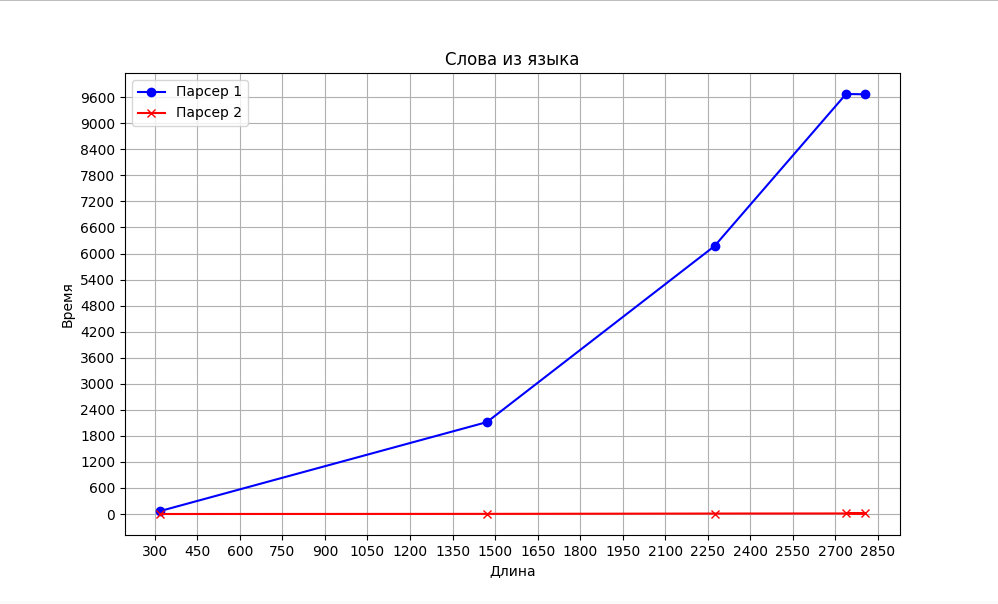
\includegraphics[width=0.5\linewidth]{img/g2.png}
    \caption{Enter Caption}
    \label{fig:placeholder}
\end{figure}
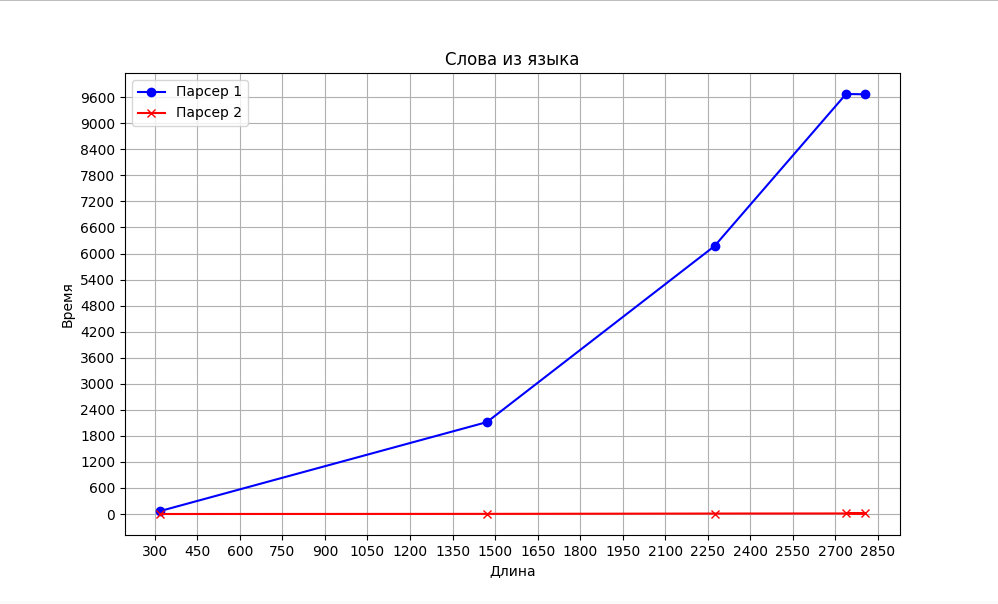
\includegraphics[width=\textwidth]{img/g2.png}
\end{figure}


\begin{figure}[!htbp]
\centering
\begin{figure}

    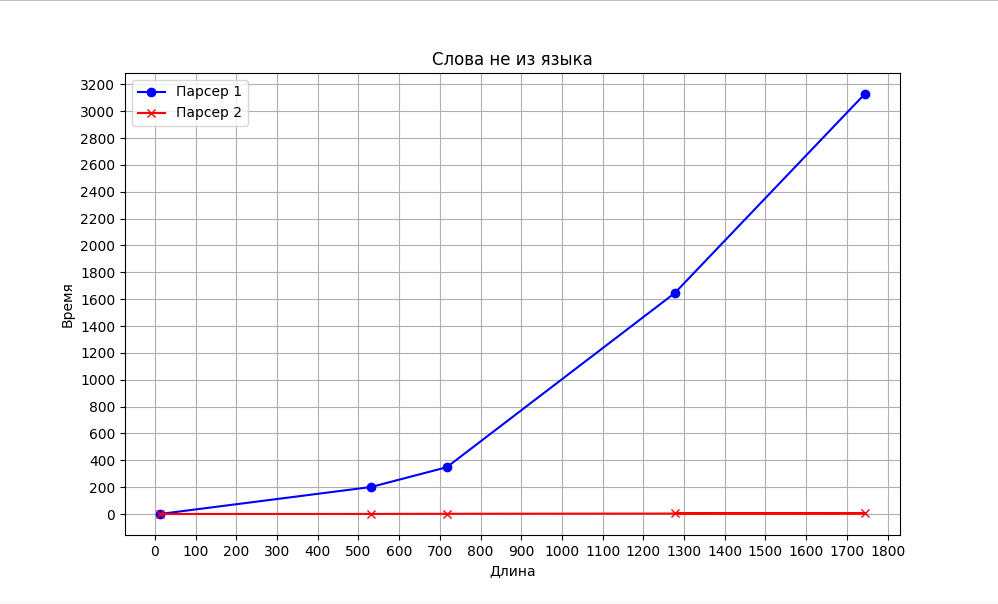
\includegraphics[width=0.5\linewidth]{img/g1.png}
    \caption{Enter Caption}
    \label{fig:placeholder}
\end{figure}
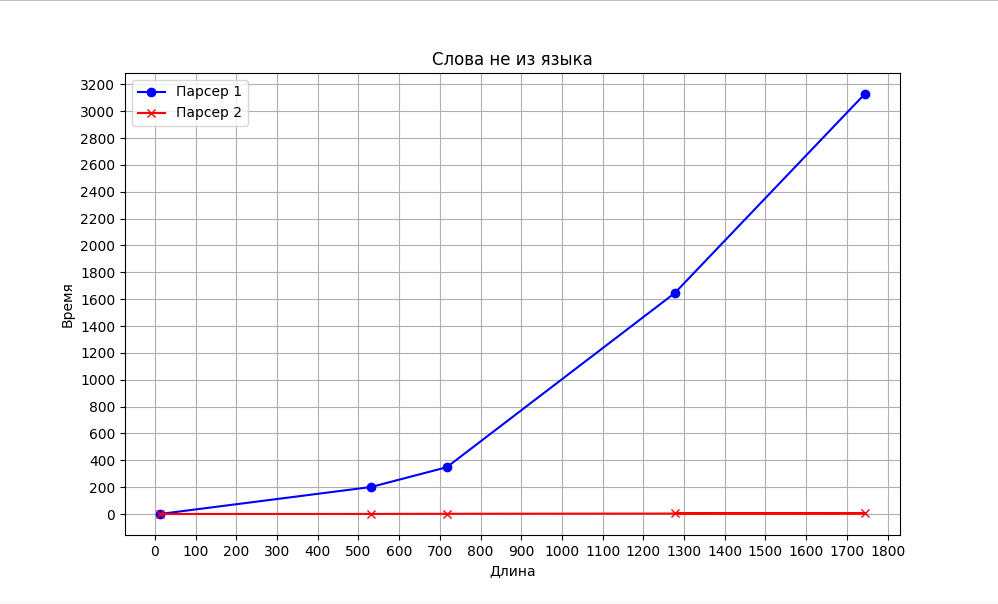
\includegraphics[width=\textwidth]{img/g1.png}
\end{figure}

\end{document}